% Here, only the tikz-code for the good example, corresponding to 'blackboard-example-1.jpg' is provided
\begin{mathstroke}[Geometric Visualization Setup]
\begin{center}
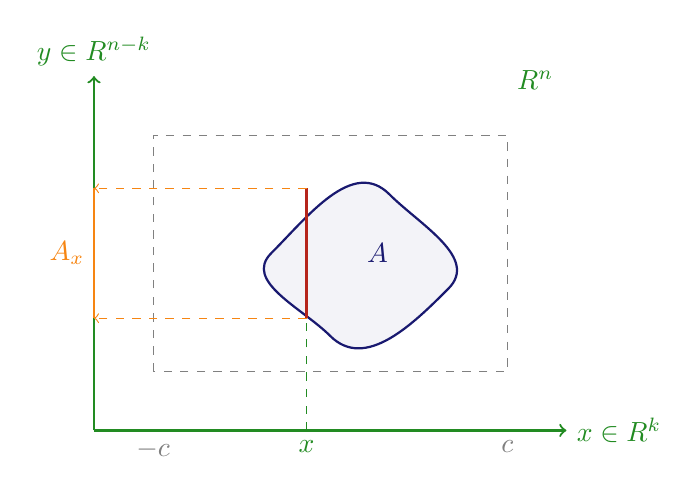
\begin{tikzpicture}[scale=1.5]
% \begin{ai-tikz-planner-invisible-content}
% 1. Background: Axes and dashed bounding box.
% 2. Midground: The set A, filled with a light color.
% 3. Foreground: The vertical slice at x and the dashed projection lines to the y-axis.
% 4. Annotations: Labels for axes, set A, slice x, and projection A_x.
% \end{ai-tikz-planner-invisible-content}
% This TikZ diagram is extracted from the blackboard at HH:MM:SS 
% This TikZ diagram was corrected/updated at the blackboard at HH:MM:SS
  % Axes with defined dimensions
  \draw[->, thick, ForestGreen] (0,0) -- (4,0) node[right] {$x \in \mathbb{R}^k$};
  \draw[->, thick, ForestGreen] (0,0) -- (0,3) node[above] {$y \in \mathbb{R}^{n-k}$};
  \node[above right, ForestGreen] at (3.5, 2.8) {$\mathbb{R}^n$};
  
  % Bounding Box [-c, c]^n
  \draw[dashed, gray] (0.5, 0.5) rectangle (3.5, 2.5);
  \node[below, gray] at (0.5, 0) {$-c$};
  \node[below, gray] at (3.5, 0) {$c$};

  % The Set A
  \draw[thick, MidnightBlue, fill=MidnightBlue!5] (1.5,1.5) to[out=45,in=135] (2.5,2.0) to[out=-45,in=45] (3.0,1.2) to[out=-135,in=-45] (2.0,0.8) to[out=135,in=-135] cycle;
  \node[MidnightBlue] at (2.4, 1.5) {$A$};

  % The Slice
  \draw[thick, BrickRed] (1.8, 0.95) -- (1.8, 2.05);
  \node[below, ForestGreen] at (1.8, 0) {$x$};
  \draw[dashed, ForestGreen] (1.8, 0) -- (1.8, 0.95);
  
  % Projection Ax
  \draw[thick, BurntOrange] (0, 0.95) -- (0, 2.05);
  \node[left, BurntOrange] at (0, 1.5) {$A_x$};
  \draw[dashed, BurntOrange, ->] (1.8, 2.05) -- (0, 2.05);
  \draw[dashed, BurntOrange, ->] (1.8, 0.95) -- (0, 0.95);
\end{tikzpicture}
\end{center}
\end{mathstroke}